\documentclass[justified]{tufte-book}

\title{Implicit Parallelism: Trying Again}

\author{Jos\'{e} Manuel Calder\'{o}n Trilla}

\usepackage{graphicx}
\usepackage{caption}
\usepackage{listings}
\usepackage{mathtools}
\usepackage{fancyvrb}
\usepackage{hyperref}
\usepackage{microtype}
\usepackage{breakcites}
%\usepackage{subcaption}
\usepackage{alltt}
\usepackage{color}

\usepackage{todonotes}
\usepackage{amsmath}
\usepackage{fancyvrb}
\usepackage{latexsym}
\usepackage{textcomp}
\usepackage{cite}
\usepackage{multicol}
\usepackage{multirow}
\usepackage{url}
\usepackage{siunitx}
\usepackage{etoolbox}

% Tufte-book imports natbib, so we can use \citet and \citep without
% importing the package
%\usepackage[round]{natbib}

\newcommand{\blankpage}{\newpage\hbox{}\thispagestyle{empty}\newpage}

%This is the stuff for semantic equations%
%%%%%%%%%%%%%%%%%%%%%%%%%%%%%%%%%%%%%%%%%%
\robustify\bfseries
\newsavebox{\sembox}
\newlength{\semwidth}
\newlength{\boxwidth}

\newcommand{\Sem}[1]{%
\sbox{\sembox}{\ensuremath{#1}}%
\settowidth{\semwidth}{\usebox{\sembox}}%
\sbox{\sembox}{\ensuremath{\left[\usebox{\sembox}\right]}}%
\settowidth{\boxwidth}{\usebox{\sembox}}%
\addtolength{\boxwidth}{-\semwidth}%
\left[\hspace{-0.3\boxwidth}%
\usebox{\sembox}%
\hspace{-0.3\boxwidth}\right]%
}
%%%%%%%%%%%%%%%%%%%%%%%%%%%%%%%%%%%%%%%%%%

\newcommand{\defineword}[2]{%
\begin{description}%
    \item{\textbf{#1}} \hfill \\%
        {#2}%
\end{description}%
}

\newcommand{\sigval}[1]{\bfseries #1}
\begin{document}

\frontmatter

%\blankpage

\maketitle

\tableofcontents
\listoffigures
\listoftables

\chapter{Introduction}

    There is a very common refrain that programmers use. It goes something like
    this: ``If you want a $[X]$ program, you must $[Y]$''. We can choose
    appropriate $X$'s and $Y$'s to prove a point about the difficulty of
    programming. Here are some common examples:

    \begin{itemize}
      \item ``If you want a fast program, you must write it in C''
      \item ``If you want an efficient program, you must write it in
                assembler''
      \item ``If you want a performant program, you must use
                cache-conscious structures''
      \item ``If you want a parallel program, you must write a parallel
                program''
    \end{itemize}

    This thesis is concerned with the last of these examples. What does it mean?
    For many, the idea that a compiler can \emph{automatically} parallelise a
    program that was written as a sequential one is a pipe-dream. This version
    of the refrain attempts to emphasise the point that utilising parallelism
    require \emph{active thought and action} by the programmer, we can not
    get parallelism `for free'.
    
    We seek to show that this is not always that case. We do this by attempting
    the inverse of the refrain: writing a compiler that is able to take a
    \emph{sequential} program and transform it into a better
    performing\footnote{This is key!} \emph{parallel} program.  A system that
    can achieve this goal is said to take advantage of a program's
    \emph{implicit}, or \emph{inherent}, parallelism.

    \defineword{Implicit Parallelism}{The potential parallelism that is present
        in a program without the need for any annotations, calling of parallel
        functions, or use of parallel libraries.}
    
    \section{Lazy Languages and Parallelism}


    \section{Thesis Roadmap}

\chapter{Parallelism in a Functional Languages}

    This chapter explores previous approaches to parallelism in a
    functional language, both implicit and explicit. We do this so that
    we may better understand the trade-offs we accept when utilising
    implicit parallelism and the difficulties involved.


    General overview of why functional programming is considered `good' for
    parallelism \citep{hughes:thesis}.
    \section{Functional Programming and Parallelism}
    \section{Approaches to Parallelism}

    When looking at parallel programming, it is important to make the
distinction between concurrency and parallelism. 
    Concurrency embodies the idea of multiple workers (threads, 
computers, agents, etc.) making progress on independent tasks. A
standard example for concurrency is a modern web-server. Each connection to 
the web-server can be thought of as an independent sub-task of the
program. The web-server does not have to be run on a multi-core 
machine for the concurrency to take place. A single-core machine
is capable of running concurrent threads through scheduling and 
context switching. 

    Parallelism describes the simultaneous execution of tasks with the purpose
of achieving a gain in performance. Tasks that
can be easily divided into independent sub-tasks can easily be made
into parallel algorithms. For example, if one wanted to compute the monthly
average temperature for a given year, each month could be computed independently.
If enough of these independent computations happen simultaneously there can
be a substantial improvement in the program's wall-clock speed. Ideally, the 
increase in performance would scale at the same rate as the available parallel
machinery (2$x$ performance with two processors, 5$x$ performance with 5 
processors). Unfortunately, there are some unavoidable factors that prevent
%this ideal from being realised \cite{hughes:thesis,HistoryOfHaskell,PFPAnIntro}. The most basic fact preventing this ideal is that the
executing machinery (whether virtual or physical) will necessarily introduce 
some overhead in the generation and management of parallel threads of 
execution \cite{PeytonJones:1992:IFL:129390}. Beyond that, it is unusual
for a program to be perfectly parallel except in trivial cases. Most parallel 
programs exhibit non-uniform parallelism and complex data dependencies. This
results in programs where parallel threads vary greatly in their processing
time and contain threads of execution that will depend on the results of other
threads. This results in threads having to wait for the result of another thread
before commencing (which is known as blocking).

 \subsection{Haskell}
    Haskell is a lazy functional language benefiting from constant development
since its inception in 1987\footnote{1987 was when the academic community
decided that an `standard' language was needed to unify the study of lazy
functional programming\cite{HistoryOfHaskell}, however, the first Haskell report was not
published until 1990 \cite{Haskell98Book}} \cite{HistoryOfHaskell,
Haskell98Book}. There have been many good introductions to
Haskell and functional programming\cite{wiki:HaskellBooks}. In this report, any 
details that may not be obvious to a non-Haskell user will be explained along 
with the code listing. 

\paragraph{Haskell Parallelism}
    The Glasgow Haskell Compiler (GHC) has extensive parallelism and
concurrency support, this is part of what makes the compiler a popular
implementation \cite{HistoryOfHaskell}.

 \subsection{Explicit Parallelism}

    The most popular Haskell compiler, GHC \cite{HistoryOfHaskell}, is able 
to compile and run parallel
Haskell programs `out of the box'. This ability is limited to the \emph{shared
memory processors}, also known as symmetric multiprocessors (SMP), that are 
nearly ubiquitous with the rise of multi-core architectures in modern CPUs. The
GHC project provides several ways to utilise parallel-capable machines. 

The first method is through the \verb=par= and \verb=seq=\footnote{While 
\texttt{seq} was introduced into Haskell for Haskell '98
\cite{Haskell98Book} it was used for many years before that
\cite{HistoryOfHaskell}. One of the earliest descriptions was by Hughes who 
introduced a \texttt{synch} combinator that
performed the same function in 1983 \cite{hughesthesis}.} combinators. The
\verb=seq= combinator has the following type.
\begin{verbatim}
        seq :: a -> b -> b
\end{verbatim}

An expression of the form \verb=seq a b= first forces the evaluation of 
\verb=a= to WHNF\footnote{For an expression to be in Weak Head Normal Form it
must be evaluated enough such that the outermost constructor is known. To say
that a function is in WHNF means that the function is partially applied.} 
and then returns \verb=b=. This allows a programmer to 
express sequential evaluation. It is important to note that 
\verb=seq= $\bot$ \verb=b= results in $\bot$. 

    It is important to realise that 
GHC's implementation of \verb=seq= does \emph{not} guarantee to force the evaluation
of its first argument. The compiler may find an optimisation that circumvents
the sequence created by the combinator. In order to provide a combinator that
\emph{does} guarantee the evaluation of the first argument before the second, 
GHC provides the \verb-pseq-\footnote{The `p' in \texttt{pseq} stands for parallel.
The idea being that parallel programs are more likely than sequential programs 
to require that \texttt{seq} guarantees its behavior.} combinator.

In the literature, the \verb=par= combinator appears in one of two forms
\cite{HistoryOfHaskell, hughesthesis}. In order to differentiate between the
two forms we will refer to the earlier version as the \emph{applicative} par, or
\verb=parAp=, and the more recent (and more common) version as \emph{Haskell} 
\verb=par=\footnote{The reason we will be referring to this as Haskell par is
because most users will know this version of the combinator from their use of
Haskell}.

Haskell \verb=par= takes the same form as \verb=seq= and has the same type
signature. The combinator takes two parameters, sparks off the first parameter
for parallelism, and returns the second. 

\begin{verbatim}
        par :: a -> b -> b

        par a b = b
\end{verbatim}

The applicative par expresses a function application whose parameter has been
sparked off to be evaluated in parallel. Semantically, this means that the
applicative par has the following form

\begin{verbatim}
        parAp :: (a -> b) -> a -> b

        parAp f x = f x
\end{verbatim}

The strictness of the function being applied can have a huge effect on the
parallelism from this combinator. In fact, we will see in section
\ref{sec:experiments} that in same cases, the compilation of the
function being applied can have large effects on \verb=parAp='s use. 

Interestingly, the version of \verb=par= that an implementation chooses does not
change of limit the expressiveness. Each version of \verb-par- can actually be
defined in terms of the other. Defining the applicative par in terms of Haskell
par gives us

\begin{verbatim}
        parAp f x = par x (f x)
\end{verbatim}

In order to define Haskell par in terms of applicative par we must use the
\verb=K= combinator

\begin{verbatim}
        K x y = x

        par x y = parAp (K y) x
\end{verbatim}

While language implementors may have strong preferences for one over the other,
there are a few good arguments for the use of Haskell \verb=par=. Haskell
\verb=par= is the simpler of the two versions, using it as an infix combinator
makes it easy to spark an arbitray number of expressions easily, 
\verb-a `par` b `par` c-, and defining applicative \verb=par= does not require
the use of any other combinators (unlike defining Haskell \verb=par= using
applicative \verb=par= which requires the \verb=K= combinator). 

    Now that we have our essential combinators we are able to define a parallel
algorithm. One of the big sellers of functional programming is the wonderfully
concise Quicksort definition

\begin{lstlisting}
        quicksort :: (Ord a) => [a] -> [a]
        quicksort (x:xs) = less ++ x:greater
            where
                less    = quicksort [y | y <- xs, y <= x]
                greater = quicksort [y | y <- xs, y > x]
        quicksort _ = []
\end{lstlisting}

The obvious way to parallelise this algorithm is to ensure that each of the two
recursive calls can be executed in parallel. This can be done by changing the second 
line to 

\begin{verbatim}
        quicksort (x:xs) = greater `par` (less ++ x:greater)
\end{verbatim}

The issue with the above is that while the left-hand side is sparked off in 
parallel, it will only be evaluated to WHNF if the spark catches. This will
result in only the first \verb=cons= of the list. The rest of the list will 
only be evaluated if/when \verb=greater= is needed\footnote{Because of 
laziness it is possible that \texttt{greater} will never be needed. An 
example would be if only the head of the sorted list is requested.}. This
fails to exploit all of the parallelism we desire and highlights the sometimes
conflicting nature of parallelism and laziness. 

    In order to help us attain the parallelism we are aiming for, we can
introduce a function \verb=force= that ensures that its parameters are evaluated
fully. As found in the textbook `Real World Haskell'' \cite{realWorld}

\begin{verbatim}
        force :: [a] -> ()
        force list = force' list `pseq` ()
            where force' (_:xs) = force' xs
                  force' []     = 1
\end{verbatim}

This function takes a list and enforces spine-strictness. As long as the list is 
not an infinite structure the use of this function is safe. With this function
in hand we could adapt our basic parallel Quicksort into a better performing one. 

An interesting point is that this definition of force can be much simpler

\begin{verbatim}
        force :: [a] -> ()
        force force (_:xs) = force' xs
              force []     = ()
\end{verbatim}

Because the function is fully saturated, the recursive call will continue
evaluating through the entirety of the list. This only goes to show that even
experts sometimes misunderstand when combinators like \verb=seq= are needed.

\begin{lstlisting}
        parQuicksort :: (Ord a) => [a] -> [a]
        parQuicksort (x:xs) = force greater `par` 
                           (force lesser `pseq` (less ++ x:greater))
            where
                less    = parQuicksort [y | y <- xs, y <= x]
                greater = parQuicksort [y | y <- xs, y > x]
        parQuicksort _ = []
\end{lstlisting}

Notice that there were a few more changes than just calling \verb=force= with
the parallel spark. By also forcing the evaluation of \verb=lesser= before
appending the two lists we ensure that both \verb=greater= and \verb=lesser=
are constructed completely. While this version of a parallel Quicksort does
execute its recursive calls in parallel it has come at a cost. First, the
resulting list is no longer lazy. Using this function for determining the head
of the resulting list would result in the entire list being computed. While
the loss of laziness can sometimes be a worthwhile trade-off (particularly 
if the entire list will be required anyway) for an increase in speed, the
second major cost is that this parallel Quicksort does not result in a faster
program!

    Despite the added functions to ensure that laziness did not get in the way
of our desired parallelism, the parallel sorting was actually slower than the
sequential sort. Running a parallel Quicksort on a two core machine, O'Sullivan
found that this algorithm actually resulted in a $23\%$ decrease in 
performance \cite{realWorld}. The reason for the slowdown comes up often in the 
design of parallel algorithms: There is a minimum amount of work a thread must
perform in order to make the expense of sparking off the thread worthwhile. This 
issue highlights what is known as granularity \cite{dutchBook}. While the sparking 
of threads is relatively cheap in a system such as GHC, there is still a cost, 
and if the amount of work a thread performs is very little, the cost may not be 
worth it. 

    One way of tackling this issue is by introducing the notion of \emph{depth}
to the function. An additional parameter can be be added to the function that
acts as a count for the depth. 

\begin{verbatim}
        parQuicksort (x:xs) depth = if depth <= 0 then quicksort (x:xs)
                                                  else ...
\end{verbatim}

    In this version we check to see if the desired maximum depth has been
reached and if so then the recursive call is to the standard sequential sorting
algorithm. If the max depth is not reached then we use the body of the
parQuicksort defined above, with the depth argument to each recursive call being
\verb=depth - 1=. The desired maximum depth is determined by the value given as
the depth argument at the top-level call of the function. This method of
controlling the granularity is a useful one and allows for easy experimentation
on the maximum depth for the problem at hand. The downside is that it
contributes yet another concern for the programmer to worry about. 

 
    Managing the granularity of a parallel program is one of the bigger
challenges facing parallel functional programming \cite{SPJ:PIFPL}. Whether
decided by the programmer (with annotations) or by the compiler implicitely, 
the question of ``is this task worth it?'' will always come up when deciding
what tasks should be sparked. 

%\footnote{We found that running a similar experiment on a 4-core machine 
%did not improve the results by much.} 

 \subsection{Implicit Parallelism}
   While explicit parallelism has many advantages and can show great performance
increases, many desire the ability to express a functional program
\emph{without} having to specify where parallelism can take place. This idea,
that parallelism can be achieved without programmer intervention, is known as
implicit parallelism. 

  \paragraph{Strictness Analysis}
    Laziness can work against our desire to exploit possible parallelism in
functional programs. Because of this, researchers have discovered that using
static analysis at compile time in order to discover strict portions of a
program can yield promising results. This analysis has been named
\emph{strictness analysis} \cite{ritabook, SPJ:PIFPL}. A trivial example is that
of the addition of two expressions, such as the fibonacci sequence. 

\begin{verbatim}
        nfib n 
            | n <= 0    = 0
            | n == 1    = 1
            | otherwise = nfib (n-1) + nfib (n-2)
\end{verbatim}

Because the \verb=(+)= function is strict in both its arguments we know that
both recursive calls to \verb=nfib= will be required. This fact, that we
\emph{know} that the arguments to a function will be required by the function,
is what enables us to exploit the parallelism that is inherent in the program. 

    Strictness analysis has
been deemed \emph{conservative} parallelism \cite{SPJ:PIFPL}. This is due to 
the idea that sparking an expression that will definitely be required by the 
program is not seen as risky. While for the most part this is true, in reality 
it depends on how the sparking is handled by the runtime. 

    There are also techniques that involve using a program's statistics gathered 
at runtime to better predict where parallelism can be exploited (Harris, Singh
2007). 

 \subsection{Semi-Implicit Parallelism}
    This section will look at things like `Strategies' to illustrate how a
programmer can write the code they want to write (for the most part) and then
use meta-techniques to make that code parallel. 

Strategies came in two waves; the first wave was introduced by Trinder et al. in
"Algorithm \(+\) Strategy \(=\) Parallelism". This incarnation of strategies is
simple to understand and easy to use effectively. 

The type declaration for a Strategy is

\begin{verbatim}
        type Strategy a = a -> ()
\end{verbatim} 

The key point to take away from this is that Strategies do not, and can not,
contribute to the end result of the computation. 

It is possible, and useful, to define strategies that do not introduce
parallelism, but instead ensure that evaluation is carried out to some degree.
For example, the strategy for doing nothing

\begin{verbatim}
        r0 :: Strategy a
        r0 _ = ()
\end{verbatim}

And for evaluating the argument to WHNF

\begin{verbatim}
        rwhnf :: Strategy a
        rwhnf x = x `seq` ()
\end{verbatim}

These strategies are not often used on their own, but are used in conjunction
with other strategies to achieve a goal. For example, applying a strategy to
each element of a list can be expressed as 

\begin{verbatim}
        seqList :: Strategy a -> Strategy [a]
        seqList strat [] = ()
        seqLIst strat (x:xs) = strat x `seq` (seqList strat xs)

        parList :: Strategy a -> Strategy [a]
        parList strat [] = ()
        parList strat (x:xs) = strat x `par` (parList strat xs)
\end{verbatim}

Both of these functions are common strategies for working on lists. In the first
case, \verb=seqList=, elements in the list are \emph{sequentially} evaluated 
using \verb=strat=. In \verb=parList=, each element is evaluated in parallel
using \verb=strat=, this gives no guarantee of the evaluation order, only that
the sparks will point to each element of the list. 

In order to use a strategy, the function \verb=using= was defined; taking an 
expression and a strategy, it bridges the gap between the specified algorithm
and the desired strategy.

\begin{verbatim}
        using :: a -> Strategy a -> a
        using x s = s x `seq` x
\end{verbatim}

This allows us to define \verb=parMap= as

\begin{verbatim}
        parMap :: Strategy b -> (a -> b) -> [a] -> [b]
        parMap strat f xs = map f xs `using` parList strat
\end{verbatim}

With this we could evaluate all the elements of a list to whatever level the
first argument specifies.

    
    %Review of Graph Reduction. Needs to focus more on the G-Machine and our
    %implementation. Will we convert to spineless G-Machine?
    \section{Graph Reduction}
    \section{History of Parallel Graph Reduction}

    1978 Turing Award winner, John Backus, used his acceptance speech to ask the
question: ``Can Programming be liberated from the von Neumann Style?''
\citep{HistoryOfHaskell}. The crux of his argument was that the traditional
and ubiquitous architecture of the day was not suitable for the eventual shift
to parallelism and the performance gains that could be achieved through
parallelism's use. This fed the
interest in novel computer architectures that would more readily support
parallelism.

More declarative languages, and particularly functional languages, were seen as
being better suited to Backus' challenge than more traditional imperative
languages. This is because many imperative languages were designed for the
simplicity of compilation. They free the programmer from repetitive
bookkeeping, such as saving registers for function calls and saving the
intermediate computations in an expression, but do not conceal all aspects of
the underlying machine. Most crucially, they allow arbitrary mutation and
side-effects. This limits the amount of parallelism possible because the result
of a function call can depend on more than values of the passed arguments.

    Work had already been carried out on non-von Neumann architectures
before that time, however, much of it was in the form of abstract machines
that functioned `on top' of the von Neumann architecture \citep{turnerHistory}.

In the early 70's the idea of graph reduction is introduced \citep{wadsworth}
and with it, the concept of lazy evaluation was ready to be formalised.
%\citep{lazyCons, HistoryOfHaskell}
Lazy evaluations has its roots in papers by Henderson and Morris, and Friedman
and Wise \citep{turnerHistory}.  People began to think of ways to better
implement graph reduction machines.  A big breakthrough for software reduction
was Turner's SKI-Combinator reduction scheme in 1979 \citep{turnerHistory,
clackbook}.

    In the 1980's we saw a great interest in parallel architectures for
functional languages. The two main conferences in the field were `LISP and
Functional Programming' (which was held on even years) and `Functional
Programming and Computer Architecture' (which was held on odd years).

    Several novel architectures were developed with the hopes that they could
surpass stock hardware in their performance. This line of research continued
through the 80's and into the early 90's \citep{Alice, GRIP, clackbook,
PFPAnIntro}.

    The G-Machine in '84 showed that lazy functional languages (which had always
been considered inefficient) could be implemented in an efficient manner on
stock hardware. However, the abstract machine could also be used in the
implementations of novel architectures \citep{Augustsson:LazyMLCompiler}.

    The 1990's saw a decline in the amount of research aimed at parallel
functional programming. This was mainly due to the results from earlier research
being less successful than had been hoped (some novel architectures did see good
results, but they could not keep up with the improvements seen in the sequential
hardware sphere) \citep{PFPAnIntro, clackbook}.

    The late 90's and the 2000's saw a resurgence in the interest in parallel
functional programming. While still constrained by the von Neumann bottleneck,
interest in this architecture is high because of the ubiquity of multi-core in
computers today. Generally, many of the techniques discussed earlier are used, but as virtual
machines abstracting away from the hardware architecture (Like GpH using GUM, or
GHC using STG-Machine) \citep{buckwheat, haskellSharedMem}.


While still suffering from the von Neumann bottleneck, the
utilisation of multiple cores has been of increasing interest. This brings us to
today.


\chapter{The Discovery and Placement of Safe Parallelism}

    New things here.
    \section{Strictness Analysis}
    Here we will describe the method by which we identify the \emph{safe}
parallelism in F-Lite programs and arrange for the evaluation of these
expressions in parallel. The \emph{strictness} properties of a function
determine which arguments are definitely needed for the function to terminate,
whereas the \emph{demand} on an argument tells us \emph{how much} of the
argument's structure is needed. \emph{Strategies} are functions that evaluate
their argument's structure to a specific depth. By analysing the program for
strictness and demand information, we can then generate strategies for the
strict arguments to a function and evaluate the strategies in parallel to the
body of the function. The strategies we generate will only evaluate the
arguments to the depth determined by the demand analysis.

In lazy languages evaluation should only occur when necessary. This apparently
sensible rule can be at odds with the goals of performance through parallelism:
if we have parallel processing resources, we wish to use them to do as much work
as possible to shorten execution time \citep{tremblay1995impact}.

Call-by-need semantics forces the compiler to take care in deciding which
sub-expressions can safely be executed in parallel.  Having a simple
parallelisation heuristic such as `compute all arguments to functions in
parallel' can alter the semantics of a non-strict language, introducing
non-termination or runtime errors that would not have occurred during a
sequential execution.


The process of determining which arguments are required for a function is known
as \emph{strictness analysis} \citep{mycroft1980theory}. Since the early 1980's
such analysis has been widely used for reducing the overheads of laziness
\citep{spjDemand}. 

\subsection{Overview}

Because we are working in a lazy language it is not always safe to evaluate the
arguments to a function before we enter the body of a function. This is easy
to see with a simple example; appending two lists\footnote{Here we have used
the na\"{i}ve recursive version, but any correct version of append will
have the same strictness properties.}:

\begin{verbatim}
    append :: [a] -> [a] -> [a]
    append []     ys = ys
    append (x:xs) ys = x : append xs ys
\end{verbatim}

\verb|append| takes two list arguments, a central question that strictness
analysis asks is: How \emph{defined} must the arguments be to \verb|append|
in order for \verb|append| to terminate?

The first hint is that \verb|append| pattern matches on its first argument.
Because the function must be able to distinguish between a \verb|(:)| and a
\verb|[]| we know that the first argument must be defined \emph{at least} to
the outermost constructor. Therefore a use of \verb|append| that is passed
$\bot$ as its first argument will result in non-termination. What about the
second argument, \verb|ys|? Determining how defined \verb|ys| must be turns
out to be impossible without taking into account the \emph{context} that
a call to \verb|append| occurs in. If the first argument is \verb|[]|
then \verb|ys| must be defined to WHNF. However the \verb|(:)| case
guards the recursive call to \verb|append| and, by extension, the use
of \verb|ys|.

The literature on Strictness Analysis is the story of determining these
properties in the general case. We start in \S \ref{sec:idealAnalysis} with
exploring the simplest Strictness Analysis, \emph{Ideal Analysis} on \emph{flat
domains}. We then show how the work was extended to \emph{non-flat domains} in
\S \ref{sec:4pointDomains}. Lastly, we show how the notion of \emph{contexts}
mentioned above are formalised by the use of \emph{projections} from Domain
Theory in section \ref{sec:projections}.


\subsection{Ideal Strictness Analysis}
\label{sec:idealAnalysis}

However, if a function uses the value of an argument within its body it is safe
to evaluate that argument before, or in parallel to, the execution of the body
of the function. In order to determine which arguments can be evaluated in this
way modern compilers use \emph{strictness analysis} \citep{mycroft1980theory}.
More formally, a function $f$ of $n$ arguments

$$
    f\ x_{1} \dots \ x_{i} \ \dots x_{n} = \dots
$$

\noindent is strict in its $i$th argument if and only if

$$
    f\ x_{1} \dots \ \bot \ \dots x_{n} = \bot
$$

What this states is that $f$ is only strict in its $i$th argument if $f$
becomes non-terminating\footnote{In this paper we use the convention that
$\bot$ represents erroneous or non-terminating expressions.} by passing a
non-terminating value as its $i$th argument.

Knowing the strictness information of a function is the first step in automatic
parallelisation. This is because if $f$ is strict in its $i$th argument we do
not risk introducing non-termination (which would not otherwise be present) by
evaluating the $i$th argument in parallel. In other words, evaluating $x_{i}$ in
parallel would only introduce non-termination to the program if evaluating $f$
with $x_{i}$ would have resulted in $f$'s non-termination anyway.

F-Lite has two primitives for taking advantage of strictness information: $par$
and $seq$.
\begin{figure}
\begin{align*}
    &seq \ :: \ a \rightarrow b \rightarrow b &&par \ :: \ a \rightarrow b \rightarrow b \\
    &seq \ x \ y = y                          &&par \ x \ y = y
\end{align*}
\caption{Semantics of \texttt{seq} and \texttt{par}.}
\label{fig:seqandpar}
\end{figure}

Both functions return the value of their second argument. The difference is in
their \emph{side-effects}. $seq$ returns its second argument only \emph{after}
the evaluation of its first argument. $par$ forks the evaluation of its first
argument in a new parallel thread and then returns its second argument; this is
known as \emph{sparking} a parallel task \citep{clack1986four}.

Strictness analysis was a very active research area in the 1980's and the
development of analyses that provide the type of strictness information
outlined above is a well understood problem \citep{mycroft1980theory,
clack1985strictness, burn1986strictness}.  However, as outlined above,
strictness analysis does not provide satisfactory information about complex
data-structures \citep{wadler1987strictness}. This can be remedied by the
use of \emph{projections} to represent \emph{demand}.

\subsection{Abstract Interpretation}

Mycroft introduced the use of abstract interpretation for performing strictness
analysis on call-by-need programs over thirty years ago
\citep{mycroft1980theory}.
Strictness analysis as originally described by Mycroft was only capable of
dealing with a two-point domain (values that are definitely needed, and values
that may or may not be needed). This works well for types that can be
represented by a flat domain (Integer, Char, Bool, etc.)\footnote{Any type that
can be represented as an enumerated type.} but falls short on more complex data
structures. For example, even if we find that a function is strict in a list
argument, we can only evaluate up to the first \verb'cons' safely. For many
functions on lists, evaluating the entire list, or the spine of the list, is
safe; canonical examples are \verb'sum' and \verb'length'.

In order to accommodate this type of reasoning, Wadler developed a
\emph{four-point domain} for the abstract interpretation of list-processing
programs \citep{wadler1987strictness}. However, when extended in the natural way
for general recursive data structures, the size of the domains made finding
fix-points prohibitively costly.

\section{Projections and Contexts}
\label{sec:projections}

So far our discussion of strictness has only involved two levels of
`definedness': a defined value, or $\bot$. This is the whole story when dealing
with \emph{flat} data-structures such as Integers, Booleans or Enumerations.
However, in lazy languages nested data-structures have \emph{degrees} of
definedness.

Take the following example function and value definitions in F-Lite

\begin{centering}
\begin{BVerbatim}
length []     = 0                   sum []     = 0
length (x:xs) = 1 + length xs       sum (x:xs) = x + sum xs

definedList = [1,2,3,4]             infiniteList = [1,2,3...

partialList = [1,2,bot,4]           loop = loop
\end{BVerbatim}
\end{centering}\\

Both \verb-length- and \verb-sum- are functions on lists, but they use lists
differently. \verb-length- does not use the elements of its argument list.
Therefore \verb-length- would accept \verb-definedList- and \verb-partialList-
(which has a non-terminating element) as arguments and still return the correct
value. On the other hand \verb-sum- \emph{needs} the elements of the list,
otherwise it would not be able to compute the sum. For this reason, \verb-sum-
only terminates if it is passed a fully defined list and would result in
non-termination if passed \verb-partialList-. Neither function would terminate
if passed \verb-infiniteList-, since even \verb-length- requires the list to
have a finite length (some functions do not require a finite list, such as
\verb-head-, the function that returns the first element in a list). With
these examples we say that \verb-length- \emph{demands} a finite list, whereas
\verb-sum- \emph{demands} a fully-defined list.

This additional information about a data-structure is extremely useful when
trying to parallelise programs. If we can determine \emph{how much} of a
structure is needed we can then evaluate the structure to that depth in
parallel.

%The first notable attempt at capturing this type of information was
%by Wadler in 1987 \citep{wadler1987strictness}. However, his approach worked
%well on lists but did not scale well to other, more complex data-structures.

The work that introduced this representation of demands was by Wadler and
Hughes \citep{wadler1987projections} using the idea of \emph{projections} from
domain theory.  The technique we use in our compiler is a projection-based
strictness analysis based on the work in Hinze's dissertation
\citep{hinze1995projection}.  Hinze's dissertation is also a good resource for
learning the theory of projection-based strictness analysis.

\section{Demand Analysis}
\label{sec:strictness}
%

In this section we provide a brief overview of the two
predominant techniques for strictness analysis: \emph{abstract interpretation}
and \emph{projection-based} analysis.  We then motivate our decision to use a
projection-based analysis.

\subsection{Projections}

This explosion in cost motivated Wadler and Hughes to propose using
\emph{projections} from domain theory to analyse strictness
\citep{wadler1987projections}.


Projection-based analysis provides two benefits over abstract interpretation:
the ability to analyse functions over arbitrary structures, and a
correspondence with parallel strategies \citep{marlow2010seq, strategies}. This
allows us to use the projections provided by our analysis to produce an
appropriate function to compute the strict arguments in parallel.

Strictness analysis by abstract interpretation asks ``When passing $\bot$ as an
argument is the result of the function call $\bot$?''. Projection-based
strictness analysis instead asks ``If there is a certain degree of demand on
the result of this function, what degree of demand is there on its
arguments?''.

What is meant by `demand'? As an example, the function \verb'length' requires
that the input list be finite, but no more. We can therefore say that
\verb'length' \emph{demands} the spine of the argument list. The function
\verb'append' is a more interesting example:

\begin{alltt}
        append :: [a] -> [a] -> [a]
        append []     ys = ys
        append (x:xs) ys = x : append xs ys
\end{alltt}

By studying the function we can tell that the first argument must be defined to
the first cons, but we cannot know whether the second argument is ever needed. However, what
if the \emph{result} of \verb'append' needs to be a finite list? For example:

\begin{alltt}

    lengthOfBoth :: [a] -> [a] -> Int
    lengthOfBoth xs ys = length (append xs ys)
\end{alltt}

In this case \emph{both} arguments to \verb'append' must be finite. Projections
can be used to formalise this type of context \citep{wadler1987projections,
hinze1995projection}.

\subsection{Semantics of Projections}

Given a domain $D$, a projection on $D$ is a continuous function
$\pi \ : \ D \rightarrow D$ that satisfies

\begin{align}
\pi \sqsubseteq ID \\
\pi \circ \pi = \pi
\end{align}

Equation (3) ensures that a projection can not add any information to a value,
i.e. all projections approximate the identity function. Idempotence (4) ensures
that projecting the same demand twice on a value has no additional effect. This
aligns with our intuition of demand. If we demand that a list is spine-strict,
demanding spine-strictness again does not change the demand on the list.

Because we want the introduction of parallelism to be semantics-preserving we
use the following safety condition for projections:

\begin{equation}
\gamma \ \circ \ f = \gamma \ \circ \ f \ \circ \ \pi
\end{equation}

Given a function $f \ : X \rightarrow Y$, and demand $\gamma$ on the
\emph{result} of $f$, projection-based analysis propagates the demand given by
$\gamma$ to the arguments of $f$. This results in the demand on the
\emph{arguments} of $f$ given by $\pi$.  The analysis aims to find the
\emph{smallest} $\pi$ for each $\gamma$, but approximating towards $ID$ (as
it is always safe to project the identity).

\paragraph{Demands on Primitives}
On unlifted base types, such as unboxed integers, there are two demands,
$ID$ and $BOT$, with the following semantics


\begin{align}
ID \ x \ &= \ x \\
BOT \ x \ &= \ \bot
\end{align}


When an expression is in a $BOT$ context it means that non-termination is
inevitable. You can safely evaluate an expression in this context because there
is no danger of \emph{introducing} non-termination that is not already present.

\paragraph{Demands on Lifted Types} Haskell's non-strict semantics means that
most types we encounter are \emph{lifted} types.  Lifted types represent
possibly unevaluated values. Given a demand $\pi$ on $D$, we can form two
possible demands on $D_{\bot}$, $\pi!$ and $\pi?$; strict lift and lazy lift
respectively. To paraphrase Kubiak et al.: $\pi!$ means we will definitely need
the value demanded by this projection, and we will need $\pi$'s worth of it
\citep{kubiak}. $\pi?$ does not tell us whether we need the value or not, but if
we \emph{do} need the value, we will need it to satisfy $\pi$'s demand.

\paragraph{Demands on Products} A projection representing a demand on a product
can be formed by using the $\otimes$ operator with the following semantics

\begin{align*}
\langle \pi_{1} \otimes \dots \otimes \pi_{n} \rangle \ \bot &= \bot \\
\langle \pi_{1} \otimes \dots \otimes \pi_{n} \rangle \ 
\langle x_{1}, \dots, x_{n} \rangle &= \langle \pi_{1} x_{1}, \dots, \pi_{n} x_{n} \rangle
\end{align*}

\paragraph{Demands on Sums} If projections are functions on a domain, then
$\oplus$, the operator that forms projections on sum-types performs the case-analysis.

\begin{align*}
[ID_{True} \oplus ID_{False}]  \ True &= True \\
[ID_{True} \oplus BOT_{False}] \ False &= \bot
\end{align*}

\begin{figure}
\begin{align*}
    d ::=&\ BOT              & \text{Bottom (hyperstrict)} \\
        |&\ ID               & \text{Top (the identity)} \\
        |&\ \langle d_{1} \otimes d_{2} \dots \otimes d_{n} \rangle   & \text{Products} \\ 
        |&\ [d_{1} \oplus d_{2} \dots \oplus d_{n}]    & \text{Sums} \\ 
        |&\ \mu\beta . d     & \text{Recursive Demands} \\
        |&\ d?               & \text{Strict Lift} \\
        |&\ d!               & \text{Lazy Lift}
\end{align*}
\caption{Abstract Syntax for Contexts of Demand}
\label{fig:ContextAST}
\end{figure}


Figure \ref{fig:ContextAST} presents a suitable abstract syntax for projections
representing demand.  This form was introduced by Kubiak et al. and used in
Hinze's work on projection-based analyses \citep{kubiak, hinze1995projection}.
We have omitted the details on the representation of context variables (for
polymorphic demands), for a comprehensive discussion we suggest Chapter 6 of Hinze's
dissertation \citep{hinze1995projection}.

In short, projections representing demand give us information about how defined
a value must be to satisfy a function's demand on that value. Knowing that a
value is definitely needed, and to what degree, allows us to evaluate the value
before entering the function.

\subsection*{Example Projections}

Because our primitives can be modelled by a flat domain (just $ID$ and $BOT$),
our lattice of projections corresponds with the two-point domain used in
abstract interpretation.

\hfill$\Box$

For pairs of primitive values, possible contexts include:
\begin{align}
[\langle ID? \otimes ID? \rangle] \label{IDPairs} \\
[\langle ID! \otimes ID? \rangle] \label{FSTPairs}
\end{align}


As Haskell's types are sums of products, pairs are treated as sums with only
one constructor.  For product types each member of the product is lifted.
Context \ref{IDPairs} is the top of the lattice for pairs, accepting all
possible pairs. Context \ref{FSTPairs} requires that the first member be
defined but does not require the second element. This is the demand that
\verb-fst- places on its argument.

\hfill$\Box$

For polymorphic lists there are 7 principal contexts; 3 commonly occurring contexts are:

\begin{align}
    \mu\beta.&[ID \oplus \langle \gamma? \otimes \beta?\rangle] \label{IDList} \\
    \mu\beta.&[ID \oplus \langle \gamma? \otimes \beta!\rangle] \label{FINList} \\
    \mu\beta.&[ID \oplus \langle \gamma! \otimes \beta!\rangle] \label{FULLList}
\end{align}


Here $\mu$ binds the name for the `recursive call' of the projection and
$\gamma$ is used to represent an appropriate demand for the element type of the
list.  An important point is that this representation for recursive contexts
restricts the representable contexts to \emph{uniform projections}: projections
that define the same degree of evaluation on each of their recursive components
as they do on the structure as a whole. The detailed reason for this
restriction is given on page 89 of Hinze \citep{hinze1995projection}. This
limitation does not hinder the analysis significantly as many functions on
recursive structures are themselves uniform.

With this in mind Context \ref{IDList} represents a lazy demand on the list,
Context \ref{FINList} represents a \emph{tail strict} demand, and Context
\ref{FULLList} represents a \emph{head and tail} strict demand on the list.

\hfill$\Box$

It will be useful to have abbreviation for a few of the contexts on lists. These
abbreviation are presented in Figure \ref{contexts}.

\begin{figure}[h!]
\begin{itemize}
    \item[] ID: accepts all lists
    \item[] T (tail strict): accepts all finite lists
    \item[] H (head strict): accepts lists where the head is defined
    \item[] HT: accepts finite lists where every member is defined
\end{itemize}
\caption{Four contexts on lists as described in \citep{wadler1987projections}.}
\label{contexts}
\end{figure}

We can now say more about the strictness properties of \verb'append'. The
strictness properties of a function are presented as a \emph{context
transformer} \citep{hinze1995projection}. 

\begin{align*}
    &append(ID) &\rightarrow &&ID!&;ID? \\
    &append(T)  &\rightarrow &&T!&;T! \\
    &append(H)  &\rightarrow &&H!&;H? \\
    &append(HT) &\rightarrow &&HT!&;HT!
\end{align*}

This can be read as ``If the demand on the result of \verb-append- is $ID$
then the first argument is strict with the demand $ID$ and the second
argument is lazy, but if it \emph{is} needed, it is with demand $ID$.

\hfill$\Box$

Following Hinze \citep{hinze1995projection} we construct projections
for every user-defined type. Each projection represents a
specific strategy for evaluating the structure, as we shall define in section
\ref{sec:proAndStrat}.  This provides us with the ability to generate
appropriate parallel strategies for arbitrary types. Using a
projection-based strictness analysis, we avoid the exponential blowup
of domains required for abstract interpretation.

\subsection*{Strategies}

With the more sophisticated information provided by projection-based analysis,
we require more than simply $par$ and $seq$. To this end we use the popular
technique of \emph{strategies} for parallel evaluation \citep{strategies,
marlow2010seq}. Strategies are designed to evaluate structures up to a certain
depth in parallel to the use of those structures. Normally, strategies are
written by the programmer for use in hand-parallelised code. In order to
facilitate auto-parallelisation we have developed a method to \emph{derive} an
appropriate strategy from the information provided to us by projection-based
strictness analysis. The rules for the derivation are presented as a
denotational semantics and can be found in our earlier work \citep{calderon}.

\section{The Granularity Problem}

We have now discussed how we find the parallelism that is implicit in our
program, but none of the analysis we provide determines whether the safe
parallelism is \emph{worthwhile}. Often static analysis will determine that a
certain structure is \emph{safe} to compute in parallel, but it is very
difficult to know when it is actually of any benefit. Parallelism has overheads
that require the parallel tasks to be substantial enough to make up for the
cost. A \emph{fine-grained} task is unlikely to require more computation than
the cost of sparking and managing the thread, let alone the potential to
interrupt productive threads \citep{hammond2000research, hogen1992automatic}.

One of the central arguments in our work is that static analysis \emph{alone}
is insufficient at finding both the implicit parallelism and determining whether
the introduced parallelism is substantial enough to warrant the overheads.

Our proposal is that the compiler should \emph{run} the program and use the
information gained from running it (even if it only looks at overall execution
time) to \emph{remove} the parallelism that is too fine-grained. By doing this
we shift the burden of the granularity problem away from our static analysis
and onto our search techniques. This way our static analysis is only used to
determine the safe parallel expressions, and not the granularity of the
expressions.

    
\chapter{Bitstring Search}

    This chapter will talk about the work on blind-search with Simon.

    \section{Introduction}
    The rest of this chapter describes our technique in more detail. Section
\ref{sec:blind-ParFunc} discuss the main background to this work: implicit
parallelism in functional languages. Section~\ref{sec:blind-Overview} provides
a worked example to illustrate the static analysis we perform to determine
potential parallelism.  We describe our empirical method and results in Section
\ref{sec:blind-Results}. Lastly, we offer our conclusions and discuss related
work in Section \ref{sec:blind-Conclusion}.


    \section{Overview}
    \label{sec:blind-Overview}
    In this section we will present a high-level overview of our technique.
This will provide the context for our discussion in the subsequent sections.

The program listed in Figure \ref{fig:tak} is the Tak program benchmark, often used
for testing the performance of recursion in interpreters and code generated by
compilers \citep{ExamplesOfRecursion}.

\begin{figure}
  \input{Blind/TakPhases/Tak.hs}
\caption{Source listing for Tak}
\label{fig:tak}
\end{figure}

After we perform our projection-based strictness analysis, and introduce the
safe \verb-par- annotations, we transform the program into a parallelised
version. The result of this transformation on Tak is listed in Figure
\ref{fig:takParred}.

\begin{figure}[!h]
  \input{Blind/TakPhases/TakParred.hs}
\caption{Source listing for Tak after analysis, transformation, and \texttt{par} placement}
\label{fig:takParred}
\end{figure}

Each strict argument is given a name via a \verb-let- binding. This is so that
any parallel, or \verb-seq-ed, evaluation can be shared between threads. When
there are multiple strict arguments (as is the case for \verb-tak-) we spark
the arguments in left-to-right order except for the last strict argument, which
we \verb-seq-. This is a common technique that is used to avoid potential
collisions \citep{strategies}. Collisions occur when a thread requires the
result of another thread before the result has been evaluated. By ensuring that
one of the arguments is evaluated in the current thread (by using \texttt{seq})
we give the paralell threads more time to evaluate their arguments, lessening
the frequency of collisions.

%This is best explained through a simple example:
%
%\begin{figure}
%\begin{center}
%\begin{BVerbatim}
%fib :: Int -> Int
%fib 0 = 0
%fib 1 = 1
%fib n = let x = fib (n - 1)
%            y = fib (n - 2)
%        in par x (seq y (x + y))
%\end{BVerbatim}
%\end{center}
%\end{figure}
%
%There are two threads interacting during the execution of \verb-fib-: The
%current thread of execution, $P$ (for parent), and the thread sparked by
%\verb-par x-, $C$ (for child). If the \verb-seq- were a \verb-par-, or absent
%entirely, in \verb-fib- then there is the possibility that $P$ would require
%\verb-x- immediately when evaluating \verb-x + y-. This would cause $P$ to
%block on $C$, awaiting the completion of \verb-x-'s evaluation. By having the
%function use \verb-seq- we ensure that productive work was accomplished even if
%$P$ needs to wait for $C$'s completion.
%
%\hfill$\Box$

%The function \verb-tak- happens to be strict in all three of its arguments.
%Therefore we lift all three arguments into a \verb-let- binding, allowing their
%results to be shared. Then we arrange the parallel evaluation of each of the
%arguments using \verb-par- and \verb-seq- annotations. The \verb-seq-
%annotation is to ensure that \verb-z'- is evaluated in the current thread, so
%that the current thread does not immediately block waiting for \verb-x'- or
%\verb-y'-.
%
While static analysis has determined that \verb-x'- and \verb-y'- can be
evaluated in parallel \emph{safely}, it does not determine whether parallel
evaluation of those expressions is \emph{worthwhile}. In order to address this
issue we take advantage of two key properties of our \verb-par- annotations:

\begin{enumerate}
    \item Each introduced \verb-par- sparks off a unique subexpression
            in the program's source
    \item The semantics of \verb-par- (as shown in Figure \ref{fig:seqandpar})
            allow us to return its second argument, ignoring the first,
            without changing the semantics of the program as a whole
\end{enumerate}

These two properties allow us to represent the \verb-par-s placed by static
analysis and transformation as a bit string. Each bit represents a specific
\verb-par- in the program AST. When a \verb-par-'s bit is `on' the \verb-par-
behaves as normal, sparking off its first argument to be evaluated in parallel
and return its second argument. When the bit is `off' the \verb-par- returns
its second argument, ignoring the first.

This allows us to change the \emph{operational} behavior of the program without
altering any of the program's semantics.



    \section{Implicit Parallelism in Functional Languages}
    \label{sec:blind-ParFunc}
    In this section we will motivate and discuss the benefits and drawbacks of
implicit parallelism in a lazy purely functional language. We will also give
a high-level overview of \emph{strictness analysis} which allows us to find safe
parallelism in lazy languages.

\subsection{Background}

Research into parallelism in lazy purely functional languages has a long
history that dates back to the early work on lazy functional languages
\citep{hughes:thesis, vGMachine, dutchBook, SPJ:PIFPL}\footnote{For a
comprehensive review we suggest \citep{hammond2000research}}. Non-strictness
makes it difficult to reason about when expressions are evaluated. This forces
the programmer to avoid the use of arbitrary side-effects. The resulting purity
means that functions in pure functional languages are \emph{referentially
transparent}, or the result of a function depends only on the values of its
arguments (i.e.  there is no global state that could effect the result of the
function or be manipulated by the function).

Purity alone is of huge benefit when dealing with parallelism. Because
functions do not rely on anything but their arguments the only communication
between threads necessary is the result of the thread's computation, which is
shared via the program's graph using the same mechanism used to implement
laziness \citep{SPJ:PIFPL}.

Laziness, while forcing the programmer to be pure (which is a boon to
parallelism), is an inherently sequential evaluation strategy. Lazy evaluation
only evaluates expressions when they are \emph{needed}. This is what allows for
the use of infinite data structures, only what is needed will be computed.

The two reductions of $sqr$ in Figure \ref{fig:eagerandlazy} illustrate the key
differences between lazy evaluation and eager, or strict, evaluation


\begin{figure}[!h]
\centering
\begin{multicols}{2}
\noindent
\begin{align*}
     \noalign{$\text{\underline{Eager Evaluation}}$}
     &sqr\ (5*5) \\
  =\ &sqr\ 25 \\
  =\ &let\ x\ =\ 25\ in\ x * x \\
  =\ &25 * 25 \\
  =\ &625
\end{align*}
\begin{align*}
     \noalign{$\text{\underline{Lazy Evaluation}}$}
     &sqr\ (5*5) \\
  =\ &let\ x\ =\ 5*5\ in\ x * x \\
  =\ &let\ x\ =\ 25\ in\ x * x \\
  =\ &25 * 25 \\
  =\ &625
\end{align*}
\end{multicols}
\caption{Eager and Lazy evaluation order for squaring a value.}
\label{fig:eagerandlazy}
\end{figure}

In the case of eager evaluation the argument to $sqr$ is evaluated
\emph{before} entering the function body. For lazy evaluation the argument is
passed as a suspended computation that is only \emph{forced} when the value is
needed (in this case when $x$ is needed in order to multiply $x*x$). Notice
that under lazy evaluation $5*5$ is only evaluated once, even though it is
used twice in the function. This is due to the \emph{sharing} of the result.
This is why laziness is often described as call-by-need \emph{with sharing}
\citep{hammond2000research}.

\medskip

In the case of $sqr$ in Figure \ref{fig:eagerandlazy}, both eager and lazy
evaluation required the same number of \emph{reductions} to compute the final
result. This is not always the case; take the following function definitions
\begin{align*}
    &bot \ :: \ Int\ \rightarrow\ Int \\
    &bot\ x\ =\ x + bot \\
    \quad & \\
    &const\ :: \ a\ \rightarrow\ b\ \rightarrow\ a \\
    &const\ x\ y\ =\ x
\end{align*}
\label{fig:botAndConst}

In an eager language the expression $const\ 5\ bot$ will never terminate,
while it would return $5$ in a lazy language as only the first argument
to $const$ is actually \emph{needed} in its body.

\medskip


This tension between the call-by-need convention of laziness with parallelism's
desire to evaluate expressions \emph{before} they are needed is well known
\citep{tremblay1995impact}. The most succesful method of combating this tension
is through the use of \emph{strictness analysis} \citep{mycroft1980theory,
wadler1987projections, hinze1995projection}.




    \section{Experimental Setup and Results}
    \label{sec:blind-Results}
    In this section we evaluate the use of search in finding an effective enabling
of \verb-par-s that achieves a worthwhile speed-up when the parellelised
program is run in a multi-core architecture.  As a reminder, the starting point
for our proposed technique is a program that was originally written to be run
sequentially on a single core; static analysis identifies potential sites at
which \verb-par- functions \emph{could} be applied; and then search is used to
determine the subset of sites at which the \verb-par- is actually used.

% The evaluation is motivated by an intended use-case for the technique: that
% an effective---not necessary optimal---placement of \verb-par-s can be found
% during the equivalent of a coffee break.

\subsection{Method}

The following four algorithm configurations were evaluated:
\begin{itemize}
	\item hill-climbing with all-on initialisation
	\item greedy with all-on initialisation
	\item hill-climbing with random initialisation
	\item greedy with random initialisation
\end{itemize}

Each algorithm configuration was evaluated for four settings of the number
cores: 4, 8, 16 and 24 cores. Each algorithm / core count combination was
evaluated against each of the seven benchmark programs described above.

Since both search algorithms are stochastic, multiple runs were made for each
algorithm / core count / benchmark combination, each using 30 different
seeds\footnote{All seeds were obtained from \url{www.random.org}.} for the
pseudo-random number generator.  For all runs, after each fitness evaluation,
the best bit string found and its fitness (the number of reductions made by the
main thread), was recorded.

In addition, the fitness (number of reductions) was evaluated for a bit string
where all bits are set to 1: this equivalent to using the static analysis
without optimisation using search.  This evaluation was made for each
combination of core count and benchmark.  Finally, the fitness was evaluated for the
sequential version of each benchmark.

\paragraph{Overheads} Our runtime system allows us to set the cost of creating
a parallel task, this models the overhead present in real systems. Using the
Criterion \citep{criterion} benchmarking library we found an approximate cost
for the creation of a \verb|par| in GHC's runtime\footnote{The code for
benchmarking the cost of a \texttt{par} is available at
\url{https://github.com/jmct/par-experiments}}. For the experiments we have
chosen an overhead of $300$ reductions for each call to \verb|par|.

\subsection{Results}

The results are summarised in Table \ref{tab:speedups}.  This table compares
the speed-up, calculated as the ratio of the medians of the reduction counts,
of hill-climbing with all-on initialisation compared to (a) the parallelisation
that would result from the static analysis without optimisation; (b) the
sequential version of the program; (c) the greedy algorithm with all-on
initialisation; and (d) the hill-climbing algorithm with random initialisation.
The speed-up is calculated as the factor by which the number of reductions is
reduced, and so values greater than 1 indicate that the program parallelised
using hill-climbing with all-on initialisation would be faster in the
multi-core environment.  Values in bold in the table indicate that differences
between the algorithms used to calculate the speed-up are statistically
significant at the 5\% level using a one- or two-sample Wilcoxon test as
appropriate\footnote{Since in the following we discuss the results for each
benchmark program, or combination of benchmark program and number of cores,
individually as well as for the entire set of results as a family, we do not
apply a Bonferroni or similar correction to the significance level.
Nevertheless we note here that most of the currently significant differences
would remain significant if such a correction were applied.}. The values in
blue are both statistically significant at the 5\% level \emph{and} exhibit a
speedup for more than 5\%. This separates the statistically significant
speedups that are unlikely to manifest on a real machine. The results for
\verb|Taut|, for example, are statistically faster, but the difference is so
minute (less than one tenth of a percent in all cases!) that the
non-determinism of a real architecture is likely to render the speedup
irrelevant.

\begin{table}
\caption[Results from using heuristic search]{The speed-up, calculated as the ratio of the medians of the reduction counts, achieved by the hill-climbing algorithm using all-on initialisation.}
\smallskip
\smallskip
\centering
	\sisetup{detect-weight=true, detect-inline-weight=math,round-mode=figures, round-precision=4}
\begin{tabular}{c c S S S S}
 	      & & \multicolumn{4}{c}{hill-climbing search speed-up compared to:} \\[0.25cm]
 SUT      & {Cores} & {\parbox{2cm}{\centering Static Parallel}} & {\parbox{2cm}{\centering Sequential}} & {\parbox{2cm}{\centering Greedy}} & {\parbox{2cm}{\centering Random Init}} \\[0.25cm] \hline
\multirow{4}{*}{MatMul}    & 4 & \bfseries\color{blue} 4.90301661707919  & \bfseries\color{blue} 1.02124759973798  &  1  &  1  \\
    & 8 & \bfseries\color{blue} 4.62464276508472  & \bfseries\color{blue} 1.02124759973798  &  1  &  1  \\
    & 16 & \bfseries\color{blue} 4.48549626511679  & \bfseries\color{blue} 1.02124759973798  &  1  &  1  \\
    & 24 & \bfseries\color{blue} 4.43914308383459  & \bfseries\color{blue} 1.02124759973798  &  1  &  1  \\
\hline
\multirow{4}{*}{Queens}    & 4 & \bfseries\color{blue} 1.08002338656061  & \bfseries\color{blue} 1.29449651880535  &  1  &  1  \\
    & 8 & \bfseries 1.04284123826334  & \bfseries\color{blue} 1.36903090592333  &  1  &  1  \\
    & 16 & \bfseries 1.01658424583816  & \bfseries\color{blue} 1.40075887342919  &  1  &  1  \\
    & 24 & \bfseries 1.00284839597168  & \bfseries\color{blue} 1.40077452594306  & \bfseries 1.000005587155  &  1  \\
\hline
\multirow{4}{*}{Queens2}   & 4 & \bfseries\color{blue} 6.47871841266272  & \bfseries\color{blue} 3.84268026498045  &  1  &  1  \\
    & 8 & \bfseries\color{blue} 6.4214444887208  & \bfseries\color{blue} 7.60677419801831  &  1  &  1  \\
    & 16 & \bfseries\color{blue} 6.26286318030988  & \bfseries\color{blue} 14.7914211715831  &  1  &  1  \\
    & 24 & \bfseries\color{blue} 6.10111087862129  & \bfseries\color{blue} 21.5370475166917  &  1  &  1  \\
\hline
\multirow{4}{*}{SodaCount} & 4 & \bfseries\color{blue} 4.23709552156544  & \bfseries\color{blue} 3.77256127760359  & \bfseries 1.00090381935946  & \bfseries\color{blue} 1.05522740981559  \\
    & 8 & \bfseries\color{blue} 3.54406724309037  & \bfseries\color{blue} 6.20691010897515  & \bfseries 1.00698493625413  & \bfseries\color{blue} 1.07054373432511  \\
    & 16 & \bfseries\color{blue} 3.10964257836354  & \bfseries\color{blue} 10.3951019801297  & \bfseries\color{blue} 1.08075042082402  & \bfseries\color{blue} 1.07197550990065  \\
    & 24 & \bfseries\color{blue} 2.80981399852391  & \bfseries\color{blue} 13.2551680242675  & \bfseries 1.00369023678455  &  1  \\
\hline
\multirow{4}{*}{SumEuler}  & 4 & \bfseries\color{blue} 1.49372579894484  & \bfseries\color{blue} 3.94797162309201  &  1  &  1  \\
    & 8 & \bfseries\color{blue} 1.48574818274656  & \bfseries\color{blue} 7.77250594496659  &  1  &  1  \\
    & 16 & \bfseries\color{blue} 1.46021192398224  & \bfseries\color{blue} 14.7739589421968  & \bfseries 1  &  1  \\
    & 24 & \bfseries\color{blue} 1.43221979480656  & \bfseries\color{blue} 20.6898343519261  & \bfseries 1  &  1  \\
\hline
\multirow{4}{*}{Tak}       & 4 & \bfseries\color{blue} 1.60884879829089  & \bfseries\color{blue} 1.55987328230559  &  1  &  1  \\
    & 8 & \bfseries\color{blue} 1.60872875931022  & \bfseries\color{blue} 3.11836989833956  &  1  &  1  \\
    & 16 & \bfseries\color{blue} 1.60840817353438  & \bfseries\color{blue} 6.22950966713651  &  1  &  1  \\
    & 24 & \bfseries\color{blue} 1.607828276573  & \bfseries\color{blue} 9.32979045709963  &  1  &  1  \\
\hline
\multirow{4}{*}{Taut}      & 4 & \bfseries 1.00030996496344  & \bfseries 1.00031731386223  & \bfseries 1.0000038116695  &  1  \\
    & 8 & \bfseries 1.00026247377892  & \bfseries 1.00038387590672  & \bfseries 1.00000088436617  &  1.000  \\
    & 16 & \bfseries 1.00026848403891  & \bfseries 1.00039382131741  & \bfseries 1.00001488189584  &  1  \\
    & 24 & \bfseries 1.00026848403891  & \bfseries 1.00039382131741  & \bfseries 1.00001488189584  &  1  \\
\end{tabular}\\
\label{tab:speedups}
\end{table}

\subsection{Discussion of Research Questions}

We can now look again at our four research questions from Section
\ref{sec:hypotheses} and determine whether our experiments have given us
meaningful results to any of them.

\paragraph{RQ1}
For most of benchmarks there is a relatively large speed-up of the
hill-climbing algorithm compared to the default parallelisation where all
\verb-par-s are enabled.  The largest speed-ups are for \verb|Queens2| where we
might expect a wall-clock run time that is more than 6 times better than the
default parallelisation.  For \verb|Queens| and \verb|Taut| the speed-ups are
closer to 1, but are in all cases statistically significant.

An interesting property regarding the speedups as compared to the static
placement is that they decrease as the number of cores increases.  This aligns
with our intuition for parallel programs. As the number of cores goes up, the
static placement \emph{gets away} with non-optimal \verb|par| placement. With
more cores, there is less contention for the resources of the machine. A
\verb|par| that does more work than its overheads is less likely interrupt
another, more productive thread. When the number of cores is lower, the
contention makes even productive \verb|par|s detrimental because they interrupt
threads that are even more productive.

We conclude that both the greedy and the hill-climbing algorithm can improve
parallel performance across a range of benchmarks and across a range of core
counts when compared to using the static placement of parallelism.

\paragraph{RQ2}
For \verb|Queens2| and \verb|SumEuler|, the speed-up compared the sequential
version of these benchmarks is almost linear: it approaches the number of cores
available.  For example, for \verb|SumEuler| on 4 cores, the speed-up compared
to the sequential version is $3.95$.  A linear speed-up is the best that can be
achieved, and so these results are indicative that our proposed technique could
be very effective in practice.  Meanwhile, for other benchmarks such as
\verb|MathMaul| and \verb|Taut|, there is little speed-up over the sequential
version of the benchmark.

\paragraph{RQ3} The results show that for most benchmarks, there is little
difference in the speed-up achieved by the hill-climbing and greedy algorithm.
(For clarity, the table shows the comparison only between the two algorithms
using all-on initialisation, but similar results are obtained when
initialisation is random.) Only for \verb|SodaCount| is there a non-trivial and
statistically significant difference between the hill-climbing and greedy
algorithm for all core sizes.  Figure \ref{fig:evals} performs a further
analysis for this research question: for two of the benchmarks, it plots the
best speed-up (compared to sequential) obtained so far by the algorithm against
the number of fitness evaluations.  For \verb|Queens2| at all core counts, the
greedy algorithm finds the same best speed-up as the hill-climbing, but finds
it in fewer fitness evaluations, i.e. the search is faster.  For
\verb|SodaCount|, the greedy algorithm finds its best speed-up in relatively
few evaluations. The hill-climber takes longer but finds a better speed-up at
all cores counts; the difference is most noticeable in the results for 16
cores. For the goal of having a compiler that provides you with a faster
program while you take a tea break, the greedy algorithm seems satisfactory.
For frequently-used benchmarks that account for a significant part of a
system's performance, the additional effort required to find the best
parallelisation using hill-climbing may be justified, but will depend on
context. In the end this is a subjective trade off, we feel that the results
support the use of the greedy algorithm unless finding the optimal solution
is absolutely necessary.


\begin{figure}[H]
\centering
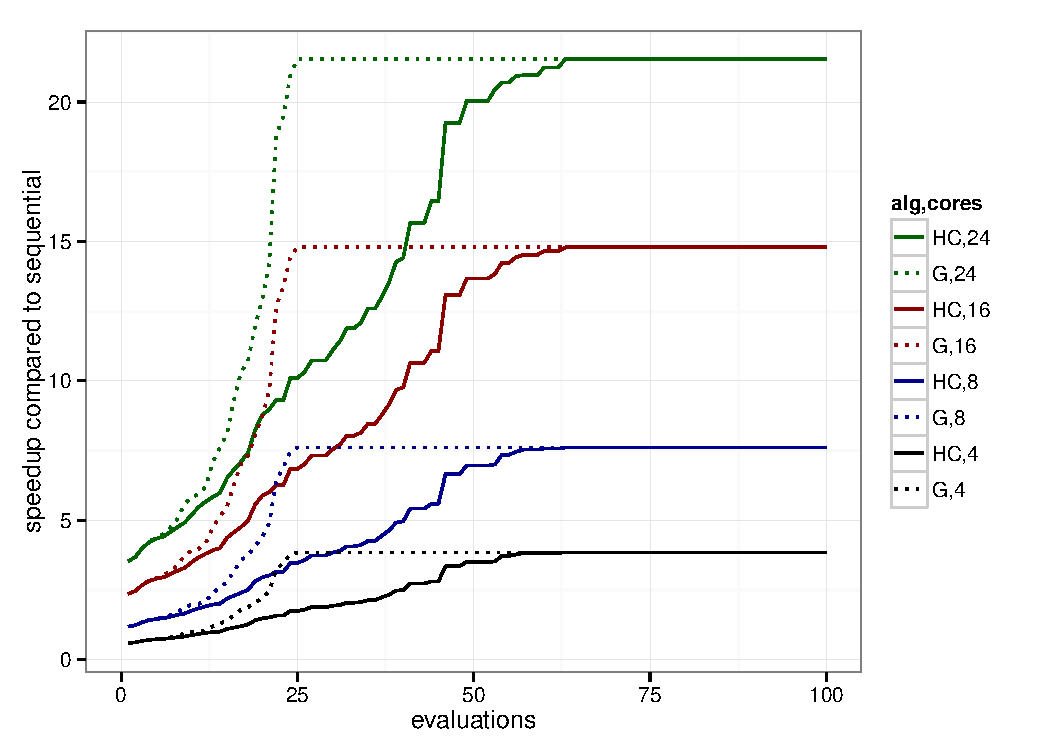
\includegraphics[scale=0.75]{Blind/Figures/speedup_by_evals_Queens2_allon_median.pdf}\\
(a) Queens2\\
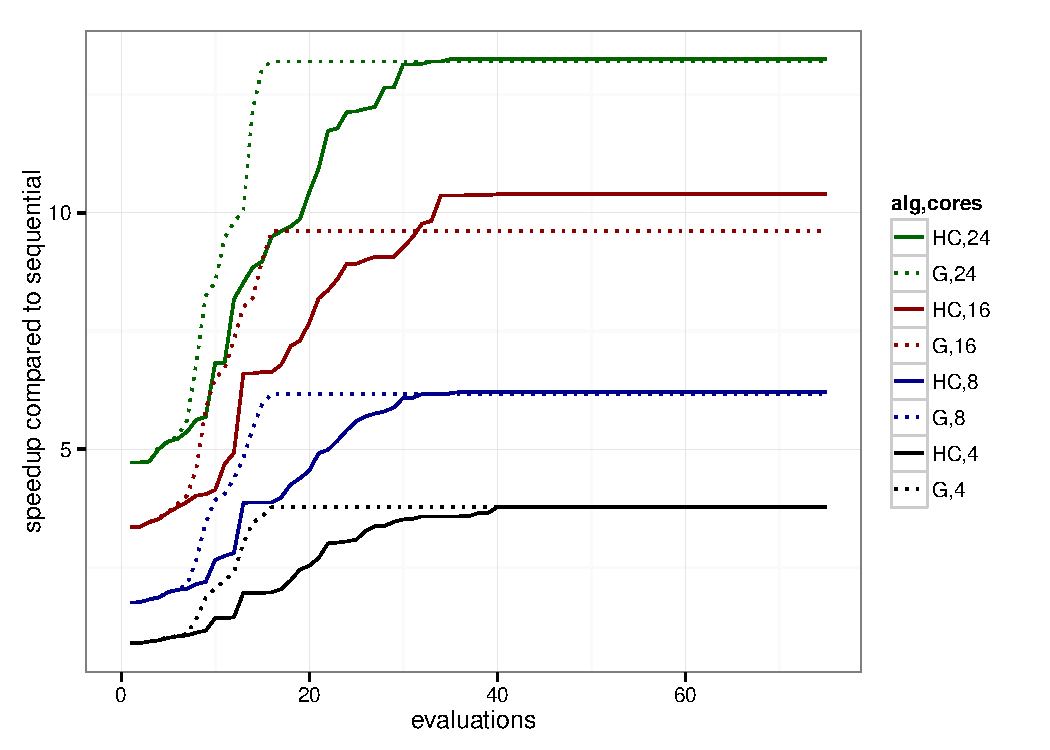
\includegraphics[scale=0.75]{Blind/Figures/speedup_by_evals_SodaCount_allon_median.pdf}\\
(b) SodaCount\\
\caption[Speedups against number of fitness evaluations for \texttt{Queens2} and \texttt{SodaCount}]{The speed-up, calculated as the ratio of the medians of the reduction counts, obtained so far by the algorithm plotted against the number of fitness evaluations. HC and G indicate the hill-climbing and greedy algorithm respectively, both using all-on initialisation. The numbers following the algorithm abbreviation indicate the number of cores.}
\label{fig:evals}
\end{figure}

\paragraph{RQ4}
For most benchmarks there is no statistically significant difference between
all-on and random initialisation.  For \verb|SodaCount|, the all-on
initialisation is slightly better for core counts of 4, 8, and 16.  This result
provides evidence that all-on initialisation may be beneficial, but requires
further investigation to confirm the generality.

\paragraph{}

The only results elided in Table \ref{tab:speedups} are the runtimes for the
greedy search with a random initialisation. This is because the random
initialisation produces inferior results in all cases and the same insight can
be gathered from studying the hill-climbing results for random initialisation.


    \section{Conclusions of Bitstring Searching}
    \label{sec:blind-Conclusion}
    We feel that this chapter has provided evidence that the combination of static
analysis and search can parallelise programs more effectively than through
static analysis alone. For some programs we are able to achieve close to linear
speed-ups which is as performant as can expected. These results are promising
for those looking to add iterative capabilities to their compiler but without
the ability to adapt the runtime system. By choosing an appropriate
representation of the available parallelism in a program, we are able to use
standard search techniques to search the possible parallel configurations.

The success of the greedy algorithm was somewhat surprising. It further
supports the idea that the vast majority of potential parallelism in any given
program does not make up for the overhead costs associated with creating and
managing that parallelism.


\chapter{Informed Search}

    New things here.
    \label{sec:informed-search}
    \subsection{Iteration}

While we do record a variety of statistics, our current approach focuses on
reduction count as a guide to determine which \verb-par- sites are beneficial
to the program.  The reasoning is simple, our motivation for parallelism is to
do more work at once, so measuring the amount of work undertaken by each thread
is likely to be a good metric.

Because we record how productive each thread in a program is and we keep track
of which \verb-par- site created each thread, we can easily visualise how useful
each \verb-par- site is. Figure \ref{fig:sumHist} gives an overview of the health
of each \verb-par--site. For each site we record the total number of reductions
carried out. The plot shows us the statistics for this data with the median
(line), inter-quartile range (IQR, box), and $\pm1.5 * $IQR (whiskers).
Statistical outliers are shown as independent points. The \verb-par-sites that
only show a line as their plot either have only one child thread (the case for
\verb-par--site 1) or have little variance in the distribution of reduction
counts.

\begin{figure}
  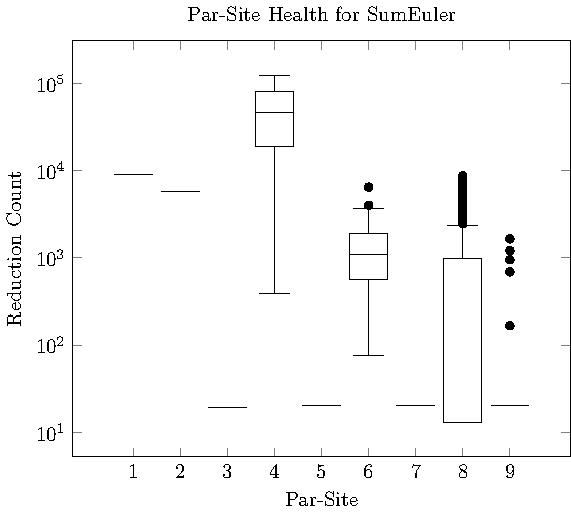
\includegraphics[width=\linewidth]{Informed/Figures/threadhealth.pdf}
\caption{Statistics on the number of reductions carried out by the threads a
\texttt{par} site sparks off}
\label{fig:sumHist}
\end{figure}

After every execution of the program, turn off the \verb'par' site whose threads
have the lowest average reduction count. In the case of the execution statistics
displayed in Figure \ref{fig:sumHist} we would disable \verb-par- site 2, allowing
us to avoid the overhead of all the unproductive threads it sparked off.  Then
repeat this process until switching a \verb'par' site off increases the overall
runtime of the program.

\section{Experimental Results}
\label{sec:results}

In this section we present some preliminary results and point out certain patterns
that appear in our data. 

First we introduce our benchmark programs and state the number of \verb-par-
sites that were introduced statically:

\subsection*{Overheads} Whether an expression is worthwhile to evaluate in
parallel is directly tied to \emph{cost} of creating a parallel task. In order
to account for this we ran all of our experiments with the simulated overhead
cost at 3 settings. We chose the upper and lower bounds based on benchmarking parallel
functions using the Criterion library \citep{criterion}.


For each program we set our runtime system to simulate 4, 8, and 16 cores.
First, let us examine Figure \ref{table10} which displays the results of setting
the cost of task creation to 10 reductions.

\begin{figure}[ht]
\centering
  \begin{tabular}{ |l||c c|c c|c c| }
    \hline
    Program & \multicolumn{2}{c|}{4-core} & \multicolumn{2}{c|}{8-cores} & \multicolumn{2}{c|}{16-cores} \\
    \hline
            & Runs & Final     & Runs & Final      & Runs & Final \\
    \hline
    SumEuler  & 6    & 3.77      & 6    & 6.84       & 6    & 10.27     \\
    Queens    & 5    & 1.30      & 5    & 1.37       & 5    & 1.41  \\
    Queens2   & 22   & 3.91      & 22   & 7.74       & 22   & 15.07   \\
    SodaCount & 3    & 2.42      & 3    & 4.72       & 3    & 8.95    \\
    Tak       & 1    & 3.39      & 1    & 6.79       & 1    & 13.58   \\
    Taut      & 4    & 1.00      & 0    & 1.00       & 9    & 1.00  \\
    MatMul    & 2    & 1.02      & 2    & 1.07       & 2    & 1.10   \\
    \hline
  \end{tabular}
\caption{Speedups relative to sequential computation when the cost of sparking
        a task is set to 10 reductions. The number of runs corresponds to the
        number of \texttt{par} sites that have been switched off.}
\label{table10}
\end{figure}

Already there are a few interesting results. \texttt{SumEuler} performs as expected and
manages to eliminate the majority of the introduced \verb-par- sites. Recalling
Figure \ref{sumLast}, the \verb-par-s that survive the iterative improvement
are the two in the \verb-main- function and the \verb-par- in \verb-mainListS2-.
The second \verb-par- in \verb-main- and the strategy \verb-mainListS2- are,
taken together, equivalent to applying \verb-parMap euler- over the input list.
When this program is parallelised explicitly, that \verb-parMap- is usually the
only addition to the program \citep{vGMachine}. It is reassuring that our
technique converges on the same result.

The two implementations of nQueens vary drastically in their improvement, with
the more symbolic solution (\texttt{Queens2}) achieving much better results. Search
problems are known to be problematic for techniques involving strictness
analysis and usually benefit from the introduction of \emph{speculative}
parallelism \citep{hammond2000research}.

\texttt{Taut} was chosen as a benchmark program specifically because the program (as
written) did not have many opportunities for parallelism. Had our technique
managed to find any useful parallelism, we would have been surprised.

MatMul is, to us, the most surprising of the results so far. Matrix
multiplication is famously parallelisable and yet our implementation
barely breaks even! Notice that of the 7 \verb-par- sites in MatMul, only
2 are being switched off. The \verb-par- setting that the iterative
improvement converged on was not the optimal setting (we know there is at least
2 superior settings). This convergence on local maxima is something we will
discuss in \S\ref{sec:conclusion}.

While the results in Figure \ref{table10} are revealing, it could be argued that
an overhead of 10 reductions to spark off a thread is unrealistically low.
Therefore we repeat the experiments with the more realistic 100 reduction
overhead (Figure \ref{table100}) and the pessimistic case of 1000 reduction
overheads (Figure \ref{table1000}).

\begin{figure}[ht]
\centering
  \begin{tabular}{ |l||c c|c c|c c| }
    \hline
    Program & \multicolumn{2}{c|}{4-core} & \multicolumn{2}{c|}{8-cores} & \multicolumn{2}{c|}{16-cores} \\
    \hline
            & Runs & Final     & Runs & Final      & Runs & Final \\
    \hline
    SumEuler  & 6    & 3.74      & 6    & 6.81       & 6    & 10.23     \\
    Queens    & 5    & 1.29      & 5    & 1.37       & 5    & 1.41  \\
    Queens2   & 22   & 3.83      & 22   & 7.57       & 22   & 14.76  \\
    SodaCount & 3    & 2.17      & 3    & 4.23       & 3    & 8.02    \\
    Tak       & 1    & 2.36      & 1    & 4.71       & 1    & 9.42   \\
    Taut      & 9    & 1.00      & 0    & 1.00       & 9    & 1.00  \\
    MatMul    & 2    & 0.93      & 2    & 1.06       & 2    & 1.09   \\
    \hline
  \end{tabular}
\caption{Speedups relative to sequential computation when the cost of sparking
        a task is set to 100 reductions. The number of runs corresponds to the
        number of \texttt{par} sites that have been switched off.}
\label{table100}
\end{figure}

The results in Figure \ref{table100} mostly align with what we would expect to
happen if creating a parallel task incurred higher overheads: we see reduced
speedup factors and adding more cores is less likely to benefit.

The key point to take away from this set of results is that while lower speedups
are achieved, the \emph{same} \verb-par- sites are eliminated in the same
number of iterations \footnote{Except for \texttt{Taut}, which in the 4-core case now
takes 9 runs to determine that there is no parallelism in the program.}.

Now we try the same experiment again but with the less realistic 1000 reduction
overhead to create a new thread.

\begin{figure}[ht]
\centering
  \begin{tabular}{ |l||c c|c c|c c| }
    \hline
    Program & \multicolumn{2}{c|}{4-core} & \multicolumn{2}{c|}{8-cores} & \multicolumn{2}{c|}{16-cores} \\
    \hline
            & Runs & Final     & Runs & Final      & Runs & Final \\
    \hline
    SumEuler  & 6    & 3.51      & 6    & 6.40       & 6    & 9.73     \\
    Queens    & 5    & 1.26      & 5    & 1.35       & 5    & 1.40  \\
    Queens2   & 22   & 3.14      & 22   & 6.22       & 22   & 12.18  \\
    SodaCount & 12   & 1.85      & 3    & 2.08       & 1    & 1.39    \\
    Tak       & 1    & 0.57      & 1    & 1.15       & 1    & 2.32   \\
    Taut      & 12   & 1.00      & 12   & 1.00       & 7    & 1.00  \\
    MatMul    & 5    & 1.00      & 5    & 1.00       & 5    & 1.01   \\
    \hline
  \end{tabular}
\caption{Speedups relative to sequential computation when the cost of sparking
        a task is set to 1000 reductions. The number of runs corresponds to the
        number of \texttt{par} sites that have been switched off.}
\label{table1000}
\end{figure}

While the speedups are now much more moderate (when there is a speedup at all)
these results are interesting for a few reasons.

In particular, the number of cores now has a greater influence on how many
\verb-par- sites are worthwhile.  \texttt{SodaCount}, for instance, now eliminates 12 of
its 15 \verb-par- annotations in the case of 4-core execution. This fits with
our intuition that when there are fewer processing units the threads require
coarser granularity to be worthwhile. In the cases of 8 and 16-core executions
we observe that fewer \verb-par- sites are disabled, reinforcing this
intuition.

MatMul also sees a jump in the number of disabled \verb-par- sites. Sadly, this
results in even worse performance for MatMul, which should be a highly
parallelisable program.

\subsection*{Static vs. Iterative}

While the results presented in Informed/Figures \ref{table10}, \ref{table100}, and
\ref{table1000} are promising for preliminary results they are based on an
admittedly simple search heuristic. Part of our argument is that static analysis
\emph{alone} is not sufficient for good gains from implicit parallelism. Figure
\ref{fig:iters} presents a selection of results that show how the iterative
improvement affects the static placement of \verb-par- annotations.

Even in the cases where the final speedup is lower than anticipated, such as
\texttt{Queens} in Figure \ref{fig:iterQueens}, the program still benefits from the
iterative improvement. \texttt{Queens2} sees the highest payoff from iterative
improvement. Many of the \verb-par-s introduced by the static analysis
do not contribute significantly to the computation even though it is
semantically safe to introduce them. The iterative loop converges on the few
\verb-par- sites that make a significant difference.

\begin{figure}[h]
    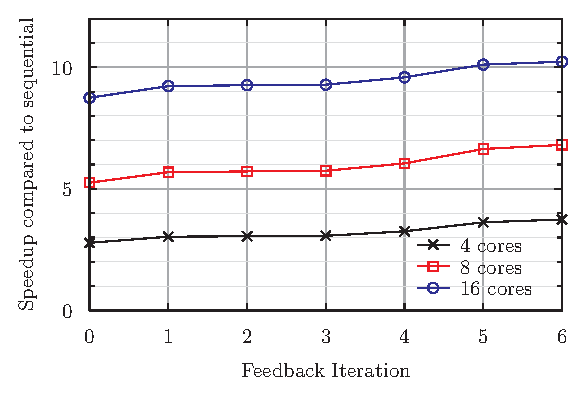
\includegraphics[scale=0.75]{Informed/Figures/IterSum.eps}
    \caption[SE]{\texttt{SumEuler} speedup}
    \label{fig:iterSum}
\end{figure}
\begin{figure}[h]
    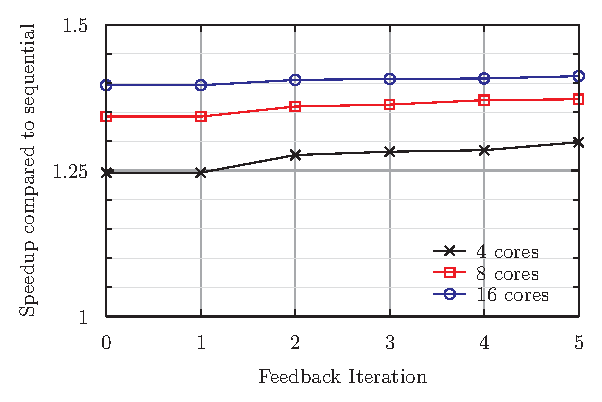
\includegraphics[scale=0.75]{Informed/Figures/IterQueens.eps}
    \caption[Q]{\texttt{Queens} speedup}
    \label{fig:iterQueens}
\end{figure}

\begin{figure}[h]
    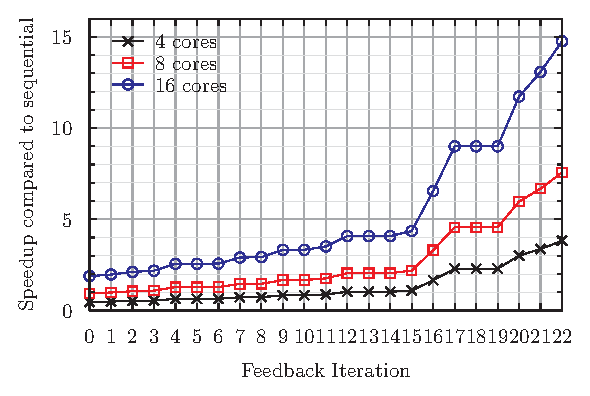
\includegraphics[scale=0.75]{Informed/Figures/IterQueens2.eps}
    \caption[Q2]{\texttt{Queens2} speedup}
    \label{fig:iterQueens2}
\end{figure}
\begin{figure}[h]
    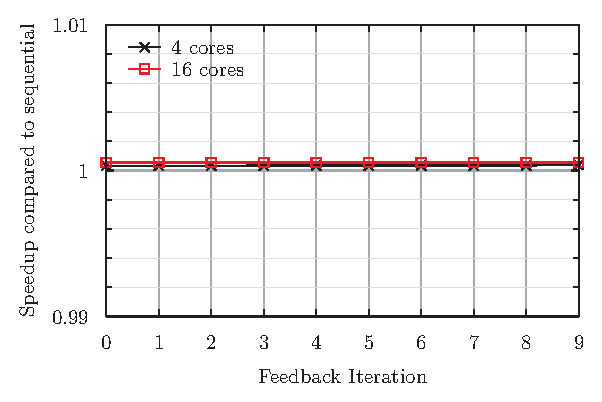
\includegraphics[scale=0.75]{Informed/Figures/IterTaut.eps}
    \caption[T]{\texttt{Taut} speedup}
    \label{fig:iterTaut}
\end{figure}


\subsection*{Comparison to GHC}

While the results above are encouraging we would like to see how the resulting
programs perform when compiled by a modern high-performance Haskell compiler.
To do this we extract the final \verb-par- settings from each program and
translate that to Haskell suitable for compilation by GHC.

For the versions parallelised by hand we use the \verb-par- placements found
in the literature \citep{vGMachine, runciman1994profiling}.

\begin{figure}[ht]
\centering
  \begin{tabular}{ |l||c c| }
    \hline
    Program & \multicolumn{2}{c|}{4-core} \\
    \hline
            & Hand   & Auto         \\
    \hline
    SumEuler  & 3.32    & 3.31      \\
    Queens    & 1.76    & 0.97      \\
    Queens2   & 2.29    & 0.61     \\
    SodaCount & 1.25    & 0.64      \\
    Tak       & 1.77    & 1.64      \\
    MatMul    & 1.75    & 0.80      \\
    \hline
  \end{tabular}
\caption{Speedups compared to the sequential program as compiled by GHC for both
         manually and automatically parallelised versions}
\label{tableGHC}
\end{figure}

As Table \ref{tableGHC} makes clear, the results are not impressive. In fact,
except for \verb-SumEuler- and \verb-Tak-, all of the parallel benchmarks
performed \emph{worse} than their sequential counterparts.

However, we feel that not all hope is lost. There are a few recurring issues in
the generated program. A common issue is that the generated strategies will not
be what forces the evaluation of a value. Take the following example as an
illustration

\begin{verbatim}
foo n = let ys = gen n n
        in par (tailStrict1 ys) (bar ys)

tailStrict1 xs = case xs of
    y:ys -> tailStrict1 ys
    []   -> ()
\end{verbatim}

In the function \verb-foo- we spark off a strategy that is meant to force the
spine of the list \verb-ys-, the catch is that GHC's \verb-par- is fast enough
for \verb-bar ys- to be what forces the evaluation of \verb-ys-. So we're
paying the overhead and reaping none of the benefits. In some programs changing
a \verb-par- like the one found in \verb-foo- to a \verb-seq- is enough to solve the
issue and make the parallel version competitive with the manually parallelised version.



\section{Conclusions}
\label{sec:conclusion}


We hope we have motivated the key design choices and ideas behind our compiler:
utilising defunctionalisation in \S\ref{sec:defunct}, and the use of
projections over other strictness analysis methods in \S\ref{sec:strictness}.
Moreover, that we have shown that there is a natural correspondence between
projections and strategies \S\ref{sec:proAndStrat} that allows us to generate
parallel strategies from the results of our strictness analysis.

While projection-based strictness analysis does provide a useful foundation for
the introduction of parallelism, the results in \S\ref{sec:results} show that
static analysis alone does not provide the desired speedups. Additionally,
Table \ref{tableGHC} shows that determining \verb-par--site health by reduction
count alone is too naive. Thread collisions that may not happen on a simulated
system are able to significantly hamper parallel performance and should be
taken into account.

\subsection{Related Work}

\subsection*{Hinze's Work on Projections} 

Much of the early work on strictness
analysis as a means to achieve implicit parallelism focused on the abstract
interpretation approach because the work on projections had not been fully
developed when implicit parallelism was a more active research area. In
particular, the work on the ``Automatic Parallelization of Lazy Functional
Programs'' \citep{hogen1992automatic} only used two and four-point domains (as
described in \citep{wadler1987strictness}) in their strictness analysis. This
limits the ability of the compiler to determine the neededness of more complex
structures.

Hinze's work on projection-based strictness analysis came after work on implicit
parallelism fell out of favour \citep{hinze1995projection, hammond2000research}. To
our knowledge we are the first to apply this work to the implicit parallelism.

\subsection{Comparison to Heuristic Search}

In the previous chapter we explored using two heuristic search algorithms to
accomplish our iterative step. While the results were promising, the ability to
examine profile data should not be underestimated. The first benefit is that
our search is guaranteed to be linear \emph{in the worst case} and usually
sub-linear, whereas even the greedy algorithm required exactly linear time.

As the programs grow larger the combinatorial explosion for the hill-climbing
will become more and more detrimental. For the hill-climbing algorithm to
terminate all neighbors to the current candidate must be explored. This means
that when a program has twenty \verb|par| sites, the \emph{last} iteration of
the hill-climbing algorithm will require twenty evaluations of the program! The
profile based technique's ability to guarantee that this program will require
\emph{at most} twenty iterations is a huge advantage.


\chapter{Conclusions}

    And.... we're done.

\backmatter

\bibliography{literature}
\bibliographystyle{plainnat}

\end{document}
